\section{Verification methods}
\label{sec:verification_methods}

Agentproof provides two complementary verification layers: (i) structural checks
over the extracted graph and (ii) temporal monitors evaluated over an event
stream.

\subsection{Structural checks}
Structural checks operate over the adjacency structure of the extracted directed
graph and the node/edge kind labels.

\paragraph{Exit reachability.}
We compute the set of nodes reachable from the entry using BFS/DFS and verify
that all declared exit nodes are included. This is $O(|V| + |E|)$.

\paragraph{Dead-end detection.}
We identify nodes (excluding \texttt{EXIT}) with no outgoing edges. Dead ends
often indicate missing transitions or incomplete error handling. This is
$O(|V| + |E|)$ with adjacency precomputation.

\paragraph{Router shape checks.}
Router nodes are expected to branch via conditional edges. We verify that all
outgoing edges from a \texttt{ROUTER} are labeled \texttt{CONDITIONAL}. This is
$O(|E|)$.

\paragraph{Human-in-the-loop presence.}
Some policies require at least one human approval node. We check whether the
graph contains any node of kind \texttt{HUMAN}. This is $O(|V|)$.

\paragraph{Tool declaration checks.}
Tool nodes should declare the tool names they may call. We flag \texttt{TOOL}
nodes with an empty tool list. This is $O(|V|)$.

\subsection{Temporal policy monitors}
Agentproof supports a small temporal policy DSL compiled into a DFA and
evaluated with constant overhead per event.

\paragraph{Event model.}
Events are dictionaries with optional fields such as \texttt{tool\_name},
\texttt{action\_type}, \texttt{decision}, and a set of \texttt{tags}. Temporal
predicates match against these fields (e.g., \texttt{tool:delete\_account}).

\paragraph{Supported DSL forms.}
The implementation supports three forms:
\begin{itemize}
  \item \texttt{G !atom} (forbidden event): violation if \texttt{atom} matches any event.
  \item \texttt{a -> F b} (interleaving constraint): once \texttt{a} occurs, \texttt{b} must occur before \texttt{a} occurs again.
  \item \texttt{a U b} (until-like safety): \texttt{a} must hold on each step until \texttt{b} occurs; otherwise a violation is triggered.
\end{itemize}
These forms are intentionally restrictive; they capture common safety patterns
while keeping compilation and evaluation simple.

\paragraph{Compilation to DFA.}
Each rule is compiled into a DFA with a small fixed number of states (three in
the current implementation). DFA transitions are implemented as a precomputed
table indexed by a bit-vector valuation of predicates. This yields $O(1)$ state
updates per event per rule.

\paragraph{Evaluation and handling.}
At runtime, each event advances the DFA state for every compiled rule. If any
rule enters a violation state, Agentproof maps the rule's configured handling
level (\texttt{warn}, \texttt{block}, \texttt{halt}, \texttt{escalate}) into an
overall decision used by the caller.

\begin{figure}[t]
  \centering
  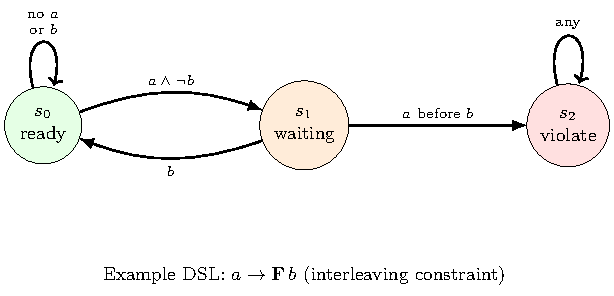
\includegraphics[width=0.85\linewidth]{figures/dfa_monitor.pdf}
  \caption{Illustrative DFA for an \texttt{a -> F b}-style interleaving constraint: after \texttt{a} occurs, \texttt{b} must occur before \texttt{a} repeats.}
  \label{fig:dfa}
\end{figure}

